


\section{ChatGLM Techniques}

In this section, we cover both the pre-training and post-training techniques we adopted and developed in ChatGLM, including model architecture, pre-training data, alignment, and All Tools. 
We have detailed technical reports introducing each of the major techniques we used to reach GLM-4. 
 

\vpara{Pre-Training Data.} 
Our pre-training corpus consists of multilingual (mostly English and Chinese) documents from a mixture of different sources, including webpages, Wikipedia, books, code, and papers. 
The data processing pipeline mainly includes three stages: deduplication, filtering, and tokenization. 
The deduplication stage improves data diversity by removing duplicated or similar documents, with both exact deduplication and fuzzy deduplication. 
The filtering stage improves data quality by removing noisy documents that contain offensive language, placeholder text, source code, etc. 
The tokenization stage converts the text into a sequence of tokens for further processing. 
The number of tokens in the pre-training data directly affects model training speed. 
To optimize this aspect, we employ the byte-level byte pair encoding (BPE) algorithm~\cite{sennrich2016neural} to separately learn the Chinese and multilingual tokens merge them with the tokens of the cl100k\_base tokenizer in tiktoken~\cite{tiktoken} into a unified vocabulary with a size of 150,000. 
In the final training set, we re-weight different sources to increase the ratios of high-quality and educational sources like books and Wikipedia. To this end, the pre-training corpus consists of around ten trillion tokens.




Throughout the four generations of ChatGLM development, our findings align with existing studies~\cite{zhou2023lima}: data quality and diversity are crucial for building effective LLMs. 
Despite the empirical lessons and insights gained, we have to date yet to identify a fundamental principle that could guide the processes of data collection, cleaning, and selection.



\vpara{Architecture.} 
The GLM family of LLMs is built on Transformer~\cite{vaswani2023attention}. 
In GLM-130B~\cite{zeng2022glm}, we explored various options to stabilize its pre-training by taking into account the hardware constraints we faced at the time. 
Specifically, GLM-130B leveraged DeepNorm~\cite{wang2022deepnet} as the layer normalization strategy and used Rotary Positional Encoding (RoPE)~\cite{su2021roformer} as well as the Gated Linear Unit~\cite{shazeer2020glu} with GeLU~\cite{hendrycks2016gaussian} activation function in FFNs. 
Throughout our exploration, we have investigated different strategies to enhance model performance and inference efficiency.  
The recent GLM-4 model adopts the following architecture design choices. 

\begin{itemize}[leftmargin=*,itemsep=0pt,parsep=0.2em,topsep=0.0em,partopsep=0.0em]
\item \textbf{No Bias Except QKV}: 
To increase training speed, we have removed all bias terms with the exception of the biases in Query, Key, and Value (QKV) of the attention layers. 
In doing so, we observed a slight improvement in length extrapolation.

\item \textbf{RMSNorm and SwiGLU}: 
We have adopted RMSNorm and SwiGLU to replace LayerNorm and ReLU, respectively. 
These two strategies have been observed with better model performance. 

\item \textbf{Rotary positional embeddings (RoPE)}: We have extended the RoPE to a two-dimensional form to accommodate the 2D positional encoding in GLM.

\item \textbf{Group Query Attention (GQA)}: 
We have replaced Multi-Head Attention (MHA) with Group Query Attention (GQA) to cut down on the KV cache size during inference. 
Given GQA uses fewer parameters than MHA, we increased the FFN parameter count to maintain the same model size, i.e., setting $d_{\mathrm{ffn}}$ to 10/3 of the hidden size.
\end{itemize}


The context length of our models was extended from 2K (ChatGLM), to 32K (ChatGLM2 and ChatGLM3), and to 128K and 1M (GLM-4). 
This expansion was achieved not only through context extension---position encoding extension ~\cite{press2022train,chen2023extending} and continual training ~\cite{xiong2023effective} on long text---but also long context alignment, enabling GLM-4 to effectively handle long contexts (Cf ~\cite{bai2024longalign} for technical details). 


\vpara{Alignment.}
Pre-training builds the foundation of LLMs while post-training~\cite{ouyang2022training} further refines these models to align with human preferences, such as understanding human intents, following instructions, and facilitating multi-turn dialogues. 
For GLM-4, the alignment is mostly achieved with supervised fine-tuning (SFT) and reinforcement learning from human feedback (RLHF)~\cite{hou2024chatglmrlhf}. 
In SFT, we find that authentic human prompts and interactions instead of template-based or model-generated responses are vital to the alignment quality. 
While SFT largely aligns the base models with human preferences, RLHF can further help mitigate  issues of response rejection, safety, mixture of bilingual tokens generated, and multi-turn coherence among others. 


For the first generation of models (ChatGLM-6B and ChatGLM-130B), the prompt-response pairs were mostly annotated by the model developers. 
For later models, the alignment data is a combination of in-house annotating data and proprietary data acquired from third parties, subject to relatively strict quality control measures. 
Similar to existing practice \cite{touvron2023llama2}, annotators are instructed to score model responses from several dimensions, including safety, factuality, relevance, helpfulness, and human preferences. 







\vpara{ChatGLM Techniques.}
Throughout the development of ChatGLM, we have introduced and will publish techniques that are used to enhance its performance. 
\begin{itemize}[leftmargin=*,itemsep=0pt,parsep=0.2em,topsep=0.0em,partopsep=0.0em]

\item \textbf{Emergent Abilities of LLMs~\cite{du2024understanding}}: 
We examined the relationship between pre-training loss and performance on downstream tasks and found that with the same pre-training loss, LLMs of different model sizes and training tokens generate the same downtream performance. We also find that on some tasks (such as MMLU and GSM8K), the performance improves beyond random chance only when the pre-training loss falls below a certain threshold.
We thus redefine emergent abilities as those exhibited by models with lower pre-training losses~\cite{du2024understanding}.

\item \textbf{LongAlign~\cite{bai2024longalign}}: 
To extend LLMs' context window size, we proposed LongAlign---a comprehensive recipe for long context alignment. 
It enables GLM-4 to process long context texts (up to 128K tokens) with performance comparable to that of Claude 2 and GPT-4 Turbo (1106). 

\item \textbf{ChatGLM-Math~\cite{xu2024chatglmmath}}: 
For the improvement of math problem solving in LLMs, we introduced ChatGLM-Math that leverages self-critique rather than external models or manual annotations for data selection. 

\item \textbf{ChatGLM-RLHF~\cite{hou2024chatglmrlhf}}: 
To align LLMs with human feedback, we introduced ChatGLM-RLHF---our practices of applying PPO and DPO into LLMs. 

\item \textbf{Self-Contrast~\cite{liu2024selfcontrast}}: 
To avoid the need for expensive human preference feedback data, we developed a feedback-free alignment strategy Self-Contrast. 
It utilizes the target LLM itself to self-generate massive negative samples for its RLHF alignment. 

\item \textbf{AgentTuning~\cite{zeng2023agenttuning}}: 
To improve LLMs' agent capabilities, we developed the AgentTurning framework with the  AgentInstruct instruction-tuning dataset that includes high-quality interaction trajectories between agents and environment. 

\item \textbf{APAR~\cite{Liu2024APAR}}: 
To improve the inference speed of LLMs for responses with hierarchical structures, we presented an auto-parallel auto-regressive (APAR) generation approach. 
It leverages instruct tuning to train LLMs to plan their (parallel) generation process and execute APAR generation. 

\item \textbf{Benchmarks}: 
We also developed several open LLM benchmarks, including 
AgentBench~\cite{liu2023agentbench} for evaluating LLMs as agents, 
LongBench~\cite{bai2023longbench} for evaluating the long context handling performance of LLMs, 
AlignBench~\cite{bai2024longalign} to measure the alignment quality of ChatGLM with Chinese language content, 
HumanEval-X~\cite{zheng2023codegeex} to evaluate HumanEval~\cite{Humaneval:abs-2107-03374} problems in programming languages beyond Python, 
as well as 
NaturalCodeBench (NCB) to measure models' capacities to solve practical programming tasks. 

\end{itemize}




\vpara{GLM-4 All Tools.}
The latest ChatGLM models are GLM-4 and GLM-4 All Tools, both of which were trained and aligned by using the techniques above. 
GLM-4 All Tools is a model version further aligned to support intelligent agents and related tasks. 
It can autonomously understand user intent, plan complex instructions, and call one or multiple tools (e.g., Web browser, Python interpreter, and the text-to-image model) to complete complex tasks. 
Figure \ref{fig:alltools-arch} presents the overall pipeline of the GLM-4 All Tools system. 
When a user issues a complex request, the model analyzes the task and plan the solving process step by step. 
If it determines that it cannot complete the task independently, it will sequentially call one or multiple external tools, utilizing their intermediate feedback and result to help solve the task.   

Built on the GLM-4's all-tools capabilities, we also developed the GLMs application platform that allows users to create and customize their own agents for specific tasks. 
The GLMs support not only the embedded Python interpreter, Web browser, text-to-image model but also user-defined functions, APIs, and external knowledge bases to more effectively address user needs. 

 



 
\begin{figure}[tb]
    \centering
    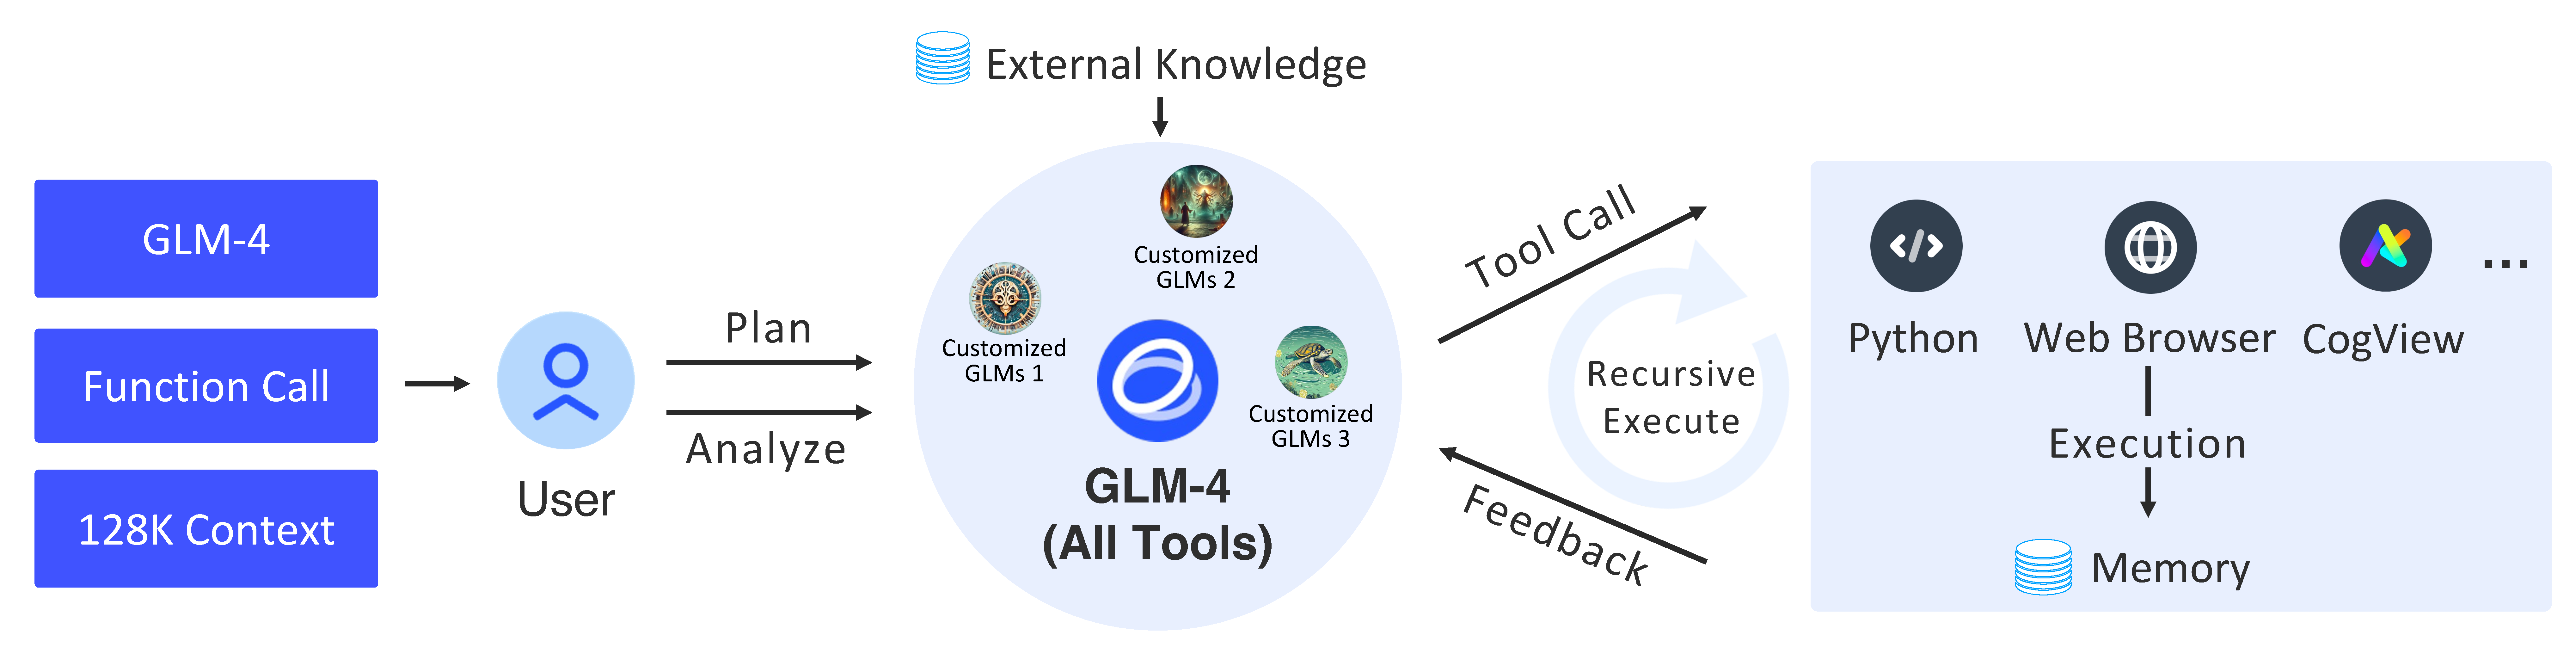
\includegraphics[width=\linewidth]{figs/glm4-alltools.pdf}
    \caption{The overall pipeline of GLM-4 All Tools and customized GLMs (agents). %\todo{aohan: Refine this figure}
    }
    \label{fig:alltools-arch}
\end{figure}


\newcommand{\eqwd}{0.1}
\newcommand{\sss}[2]{\shortstack[c]{#1\\{#2}}}
\newcommand{\ddd}[2]{\shortstack[c]{#1\\\tiny{#2}}}





